\chapter{Presentación de los datos, Análisis, Discusión}



% Definiciones

%\subsection{Conceptos y Medición}
\section{Conceptos e Indicadores}

En esta sección se explican los conceptos teóricos utilizados y sus indicadores. Posteriormente se detallan las fuentes de datos, el calculo del indicador y sus problemas. Los conceptos claves son la PEA, vacantes, desempleo y pib?? 
En cuanta la PEA y desempleo existe consenso en cuanto a su definición y medida, si bien cada país puede definir ciertas variantes que complejizan su comparación a nivel teórico no suele existir discrepancia, ya que, se suelen seguir las recomendaciones del CIET.
Sin embargo, tanto la definición como la medición de las vacantes laborales es un campo menos entendido. Primero porque no existe una definición universal de que considerar como vacante y segundo porque su medición es complicada y problemática.
% Citar a Etsby

% 1. PEA
%\subsubsection*{PEA}

El INE sigue las recomendaciones de la Conferencia Internacional de Estadísticos de Trabajo (CIET)\footnote{El CIET sigue las recomendaciones del SCN, el cual sigue el criterio de la frontera de posibilidades de producción. Según lo anterior las actividades que quedan por fuera son exclusivamente actividades de producción de servicios, los servicios excluídos son los producidos por los miembros del hogar para el consumo final propio del hogar, producidos por el trabajo voluntario desde los hogares con destino a otros hogares. Las actividades excluídas son limpieza y pequeñas reparaciones del hogar, cocinar para los miembros del hogar, tareas de cuidado y educación de los miembros del hogar, transporte de los miembros del hogar. La PEA se utiliza como un sinónimo de fuerza de trabajo}, quien define a la PEA como:

\begin{center}
\begin{minipage}{0.95\linewidth}
	\vspace{1pt}%margen superior de minipage
	{\small
	La población económicamente activa abarca todas las personas de
	uno u otro sexo que aportan su trabajo para producir bienes y servicios
	económicos comprendidos dentro de la frontera de producción, según
	la definición de los mismos contenida en la última versión del Sistema
	de Cuentas Nacionales (SCN), durante un período de referencia
	especificado. De acuerdo con el SCN 2008, la producción de bienes y
	servicios relevantes incluye toda la producción de bienes, la producción
	de servicios de mercado y no de mercado, y la producción destinada al
	autoconsumo final en el hogar de los servicios domésticos producidos
	mediante el empleo remunerado de personal doméstico
	}
%	\begin{flushright}
%		(\citeauthor{Coulouris}, \cite{Coulouris}: 10)
%	\end{flushright}
	\vspace{1pt}%margen inferior de la minipage
\end{minipage}
\end{center}

En el caso uruguayo el límite etario inferior se fija en 14 años, y el período de referencia es la semana anterior a la encuesta. La persona debe tener al menos una ocupación en la cual realizar esfuerzo productivo o que sin tenerla la busca activamente en el período que es encuestado. Se incluyen a los miembros de la sociedad civil y fuerzas armadas \cite{INE2018}. Que el límite para fijar la PEA sea a elección dificulta la comparabilidad entre países, a modo de ejemplo en Argentina es 16 años, Brasil 10, Colombia 9, Paraguay 10, Cuba 17 y Perú 14.

%Las personas inactivas son aquellas que no aportan su trabajo para producir bienes o servicios económicos y no buscan trabajo. Se clasifica en las siguientes categorías: personas que se ocupan solamente del cuidado de su hogar, estudiantes, jubilados, pensionistas o rentistas.


% 2. Desempleo
%\subsubsection*{Desempleo}
En cuanto al desempleo existe consenso por parte de países y autoridades en seguir las recomendaciones del CIET para su definición y medición. Sin embargo, la misma deja abierto a cada país el período relevante a considerar para catalogar a una persona como ocupada o desocupada, generando una diferencia en la intensidad de búsqueda\cite{Elsby2015}, relevante, ya que, puede generar subestimación en la duración del desempleo en hasta un 8\%\cite{Poterba}. Además la definición de PEA si bien compartida, presenta diferencias, por ejemplo, en los límites inferiores lo cual se traslada a la definición y medición de la tasa de desempleo. Sin embargo, la diferencia entre desempleados y personas fuera de la fuerza de trabajo son significativas, ya que, las primeras es más probable que transiten al empleo \cite{Flinn y Heckaman}.

En Uruguay, el desempleo se entiende como aquellas personas que buscan trabajo remunerado activamente pero no logran obtenerlo. Según el \cite{INE2019} 
\begin{center}
	\begin{minipage}{0.95\linewidth}
		\vspace{1pt}
		{\small
Se considera como desempleado a toda persona que durante el período de referencia considerado (última semana) no está trabajando por no tener empleo, que lo busca activamente y está disponible para comenzar a trabajar ahora mismo. Por definición, también son desocupados aquellas personas que no están buscando trabajo debido a que aguardan resultados de gestiones ya emprendidas y aquellas que comienzan a trabajar en los próximos 30 días.}
		\vspace{1pt}
	\end{minipage}
\end{center}
% Para poner comillas ``....''
 


%\subsubsection*{Vacantes}
Distinto es el caso de las vacantes laborales, dado que no existe una definición compartida a nivel conceptual. Según \cite{Abraham1983} una vacante debe verse como una demanda insatisfecha por parte de la empresa. Sin embargo, según \cite{Elsby2015} esto presenta tres problemas, el primero es que puede resultar díficil identificar el recurso ocioso en una empresa. El segundo, es la dificultad para medir la producción no llevada a cabo debido a la ausencia del puesto. Tercero, las empresas pueden contratar anticipandose a una posible apertura de posición y la misma puede variar por sector de actividad, por ejemplo, \cite{Myers1966} identificando algunos problemas conceptuales y de medición de vacantes encuentra que un 10\% de los avisos laborales se llenan antes de que el empleado actual deje la firma, y que las vacantes son más numerosas en las industrias manufactureras durables. En la medida que aumentan cambios tecnológicos sesgados hacia trabajos de mayor calificación, esto podría aumentar.

Las dificultades pueden agravarse dependiendo del sector de actividad y la tecnología de producción. Si suponemos, un sector agrario con tecnología de producción (la L, no me acuerdo) dada la relación uno a uno es fácil observar y cuantificar el perjuicio por el recurso ocioso. Pero en el caso de una línea de producción en una fábrica o en el sector servicios, la tarea se complejiza.

Como forma de operacionalizar el concepto, se sigue la definición del Job Openings and Labor Turnover Survey (JOLTS), que plantea la existencia de una vacante cuando el trabajo puede empezar en los próximos treinta dias y el empleador recluta por fuera de su establecimiento. Esto plantea la problemática que los tiempos de reclutamiento pueden ser mayores a dicho lapso y heterogeneos dependiendo de la posición, sector y temporada. Es razonable pensar que un proceso de selección de un gerente sea más extenso que el de un asistente, a la vez que los procesos de selección para contrataciones zafrales sean más rápidos que los no zafrales.





La construcción del índice tiene como base al Conference Board Help Wanted OnLine (HWOL) de EEUU, en base a \cite{Barnichon2010, Shimer2005} se observa que es un proxy confiable respecto del Job Openings and Labor Turnover Survey (JOLTS, calculado por el Bureau of Labor Statistics).  

Sin embargo, el caso uruguayo presenta particularidades de hacer notar. Hasta la década del 2000 prácticamente la única fuente existente de avisos laborales en papel fue el El Gallito, por lo cual basta con recabar dicha información para tener una muestra representativa de los avisos laborales. Sin embargo, con la revolución de internet comienza a perder representatividad. A partir de allí el problema se divide en 3: 1) Cuánta representatividad pierde 2) A partir de año comienza a perderla 3) Para responder 1 y 2, es necesario definir que otras fuente relevantes aparecen y definir la población de avisos a utilizar, la cual debe ser representativa de todos los portales laborales.


Según el \cite{JOLTS} una vacante disponible debe cumplir que 1) La posición especifica exista 2) El trabajador pueda comenzar en no más de 30 días 3) El empleador busqué activamente fuera del establecimiento la vacante.\footnote{Traducción propia}


% Desempleo

\section{Fuentes}
% Vacantes Laborales

% Fuentes de datos
\subsubsection*{INE}

Del INE se obtiene la tasa de desempleo para el departamento de Montevideo desde 1981 hasta 2019.
La Encuesta Continua de Hogares desde 1980 hasta 2018, de la cual se usa una versión compatibilizada por parte del IECON.

% El gallito
\subsubsection*{Gallito}
Primero, se obtienen los datos de \cite{Urrestarazu1997}, quien utiliza la serie de vacantes construida por \cite{Rama1988} en base a las publicaciones semanales de el diario El País, sección gallito, ministerio de trabajo y seguridad social (MTSS) y Banco Central del Uruguay (BCU) con lo cual contruye una serie trimestral entre 1978-1987\footnote{La serie construida por Rama une 3 fuentes que miden distintas poblaciones, la  X e Y son de carácter nacional mientras la J es departamental para Montevideo, el autor supone que no genera sesgos relevantes. Lo cual se demuestra más adelante}. Urrestarazu obtiene por parte de El País las publicaciones semanales entre 1989 y 1995, estima la cantidad de avisos entre 1988 y 1989 y calcula un índice de vacantes laborales de frecuencia trimestral desde 1978 hasta 1995, siguiendo la misma formula de Rama:\footnote{Para obtener la cantidad de avisos en el 1987 realiza un supuesto de aviso promedio, explicar en detalle.}.
% Los detalles de la unión de urrestarazu a un footnote
\begin{equation}
v_t = \frac{\frac{a_t}{a_0}}{\frac{PEA_t}{PEA_0}}
\end{equation}

Segundo, se recaba de forma exhaustiva los avisos laborales existentes en las publicaciones semanales de el diario El País sección 'El Gallito' entre octubre de 1995 y agosto de 1998. Además de los trimestres en los años 1999, 2000, 2009, 2010, 2012, 2013.

Tercero, se agrega una base de datos confidencial entregada por el diario El País entre 2013 y 2018 con un contenido exhaustivo de avisos laborales publicados.

Finalmente, se realiza scraping de la página web el gallito entre 2018 y 2019 de forma mensual o bi-mensual.

\subsubsection*{CERES}
Se utilizan los datos de El Centro de Estudios de la Realidad Económica y Social (CERES) \cite{Ceres2012}, quien construye un índice de vacantes laborales llamado 'Índice Ceres de Demanda Laboral (ICDL)' desde agosto de 1998 hasta  xxx de 2014 de frecuencia mensual. Los datos conseguidos están corregidos por factores estacionales\footnote{Explicar su problemática}, pero no se detalla el filtro aplicado a la serie. Tampoco es especificada la fuente de la cual se obtienen.
Dada la falta de información, se contrasta con otras fuentes de información. Para ello se utilizan los datos generados por \cite{Alma2011}, base de datos facilitada por los autores. Con ella se construye un índice de frecuencia anual, el cual se compara con el ICDL también anualizado. Se observa un comovimiento y correlación de 97\%. También se analizan ambas series en tasas de crecimiento, mediante una transformación logarítmica y posterior diferencia, ambas muestran resultados similares con una correlación de 90\%.
Adicionalmente, los avisos de el Diario El País, recolectados entre 1999 y 2013, se utilizan como muestras de forma tal de corroborar la hipótesis que el ICDL debe estar generado a partir de publicaciones de el Diario El País\footnote{text}.
% Agregar imagen
% Agregar fórmula
% Agregar en el anexo los métodos de imputación utilizados.

\subsubsection*{Buscojobs}
Se recaba la cantidad de publicaciones mensuales publicadas por el portal buscojobs entre 2007 y 2019. Para el periodo 2007 a 2018 se obtienen muestras por mes y en cada mes, las cuales son promediadas mensualmente obteniendo la cantidad de avisos mensuales, dichos datos son obtenidos a través de la página web waybackmachine. 
Para el año 2019 se realiza scraping del portal buscojobs.

\subsubsection*{Computrabajo}
Finalmente se extraen todas las publicaciones mensuales disponibles publicadas en el portal laboral computrabajo entre 2003 y 2018 a partir de waybackmachine y avisos laborales entre 2018 y 2019 mediante scraping del portal computrabajo. La particularidad de este portal es que la cantidad de avisos publicados que se observa no se corresponde con la cantidad de avisos publicados en los últimos 30 días debido a que dicho portal mantiene avisos por más de 60 días, inclusive. 

Nota del scraping. Es de hacer notar, que las tres páginas web de las cuales se extrajeron los datos difieren en cuanto a la estructura con la cual presentan los avisos laborales, pese a ser el mismo aviso se presenta de forma diferente y se pueden encontrar variaciones en cuanto a la información brindada. Por ejemplo, puede que el nombre del puesto y la empresa difieran levemente. En otras ocasiones no se brinda información respecto a la empresa, o se hace referencia a ''importante empresa''. Para poder identificar empresas compartidas por portales, primero se limpia el texto, se borran 'stopwords', se buscan patrones similares y finalmente se hace un filtro manual del cual se mapean 452 valores contenidos en una matriz de dimensión $\Re^{207*6}$ hacia un vector $x$ de dimensión $\Re^{207}$. 

\section{Construcción}

Notación: \newline
$a_t$ = avisos totales año t \newline
$a_0$ = avisos totales año 0 \newline
$pea_t$ = Población Económicamente Activa año t \newline
$pea_0$ = Población Económicamente Activa año 0 \newline
$v_t$ = índice de vacantes año t \newline
$v_0$ = índice de vacantes año 0 \newline
$v_m$ = índice de vacantes urrestarzu, años 1980-1995 \newline


El objetivo es obtener una aproximación de la cantidad de avisos totales, por ello primero es necesario obtener $a_t$ desde el índice de vacantes Urrestarazu. Sin embargo, la base de dicho índice es 1980 y los datos disponibles en el trabajo son desde 1981 en adelante. El índice esta expresado en función de la PEA:
\begin{equation}
v_t = \frac{\frac{a_t}{a_0}}{\frac{PEA_t}{PEA_0}}
\end{equation}

No se conoce $a_0$ ni $PEA_0$, ni se tienen datos de 1980. Por lo cual, se siguen los siguientes pasos:

1. Obtener $a_t$ en algún punto: $a_{1995_q4}$\footnote{La cantidad de avisos laborales del cuarto trimestre de 1995, fueron obtenidos a partir de las publicaciones del diario El País, sección Gallito}.
2. Imputar la PEA hacia atrás, obteniendo $pea_{t=0}$.
3. Obtener $a_{t=0}$:
$v_t$ = $(a_t/pea_t)/(a_{t=0}/pea_{t=0})100$.
4. Obtener la base $\alpha$ = $a_{t=0}$/$pea_{t=0}$.
5. Imputar las vacantes hacía atras.
6. Calcular la serie de avisos

Se opta por realizar una predicción hacia atrás, planteando un modelo básico estructural (citar Harvey, Hamilton, Bishop, etc) mediante un filtro de Kalman suavizado (citar..).\footnote{Se plantearon formulaciones alternativas, como imputación mediante filtro de kalman sin suavizar, con 3 tipos de modelos estructurales: local-level, trend, básico estructural, además de modelos arima representados en la formulación de espacio estado.}

A continuación se une la serie de avisos 1980-1995 con los avisos recolectados entre 1995 y 1998, dado que se utilizo $a_{1995_{q4}}$ las series coinciden y pueden ser combinadas sin realizar ningún calculo adicional, la serie obtenida se denota $a_{um}^{80-98}$.

Luego, se utiliza la serie de ceres, $a_{ceres}^{98-14}$, de frecuencia mensual y sin factores estacionales\footnote{Como se mencionó, no se conoce el método de desestacionalización, solo se sabe que las notas metodológicas indican "", sin embargo, por los análisis realizados lo más verosímil es que la serie publicada sea la tendencia-ciclo, en la sección siguiente se responden dichas críticas}. Se trimestraliza, y se realiza la unión, ambas series coinciden en el período compartido, se obtiene $a_{umc}^{80-14}$.

El paso siguiente fue la creación de una serie mensual de publicaciones sin avisos repetidos por link, utilizando los datos proporcionados por el diario El País, entre 2013 y 2018. Dicha serie se une con los avisos obtenidos para el año 2019 mediante el scraping web de la página web el gallito. Posteriormente se trimestralizan los datos.

A continuación, se utilizan los avisos laborales facilitados por el diario El País para el período 2013-2019, con ellos se construye una serie trimestral de la cantidad de publicaciones.
Dichos datos es la variable no observable que deseamos cuantificar en los períodos previos pero que observamos con errores de medición, por ello lo denotamos $\tilde{a_t}$. De forma de obtener, cuanto difieren los avisos en papel de los avisos de la base de datos, se muestrean los siguientes trimestres: $a_{q4}^{13}$, $a_{q1}^{14}$, $a_{q2}^{14}$, $a_{q3}^{14}$, $a_{q4}^{14}$\footnote{En todos los casos existen semanas, donde la publicación semanal no estaba disponible. Por ello, se modelizaron serie de frecuencia semanal las cuales fueron imputadas mediante la modelización de un modelo básico estructural estimado por un filtro de kalman suavizado}. Como se puede observar en la TABLA-NUMERO la diferencia entre $\tilde{a_t}$ y ${a_t}$ es significativa. Por ello, se repondera la serie $a_{umc}^{80-14}$ en base al promedio de los avisos $a_{q2}^{14}$, $a_{q3}^{14}$, $\tilde{a}_{q2}^{14}$, $\tilde{a}_{q3}^{14}$ sin duplicar. 

\begin{table*}
	
	\caption{\label{tab:}Tabla de avisos laborales}
	\centering
	\resizebox{\linewidth}{!}{
		\begin{tabular}[t]{c|c|c|c|c|c|c|c|c}
			\hline
			avisos\_bd\_s\_dup & avisos\_bd\_c\_dup & avisos\_papel & fecha & ratio\_s\_dup & ratio\_c\_dup & diferencia\_s\_dup & pct\_s\_dup & pct\_c\_dup\\
			\hline
			8342 & 8403 & 12619.95 & 2013-10-01 & 1.512821 & 1.501839 & 4277 & 0.6610167 & 0.6658503\\
			\hline
			9228 & 9478 & 11631.89 & 2014-01-01 & 1.260499 & 1.227251 & 2403 & 0.7933365 & 0.8148292\\
			\hline
			7720 & 7918 & 10049.00 & 2014-04-01 & 1.301684 & 1.269134 & 2329 & 0.7682356 & 0.7879391\\
			\hline
			7187 & 7515 & 9703.00 & 2014-07-01 & 1.350076 & 1.291151 & 2516 & 0.7406988 & 0.7745027\\
			\hline
			6897 & 7212 & 9830.00 & 2014-10-01 & 1.425257 & 1.363006 & 2933 & 0.7016277 & 0.7336724\\
			\hline
	\end{tabular}}
\end{table*}

Además, dada la diferencia que se observa entre los muestreos y la serie de ceres a partir del año 2012, se considera dicha serie hasta el año 2012, y se imputan los valores trimestrales $a_{q2}^{12}$, $a_{q3}^{12}$, $a_{q4}^{12}$, $a_{q2}^{13}$. Se divide la serie en estaciones (trimestres) y se realizan imputaciones en cada serie por separado, utilizando el filtro de kalman como método de estimación. De esta forma se obtiene la serie final correspondiente al diario El País sección gallito Luis.
% Agregar gráfico.


% Serie de Buscojobs
Los publicaciones laborales del portal buscojobs se recaban desde 2007/06 hasta 2018/12 a través de la página web waybackmachine. Se contabilizaron todas las publicaciones mensuales encontradas que hacen referencia al total de avisos publicados, los cuales son promediados mensualmente. Es decir, cada punto refiere a un año-mes y el total de avisos de publicados en dicho momento.

En el año 2019, se realiza scraping sobre el portal buscojobs, del cual se extraen todos los avisos laborales disponibles, la extracción de datos se realiza de forma mensual o bimensual y se obtiene la información completa de cada aviso.
La serie se modela con frecuencia mensual y los valores faltantes son imputados removiendo el componente estacional de la serie, imputando la serie desestacionalizada y luego agregando el componente estacional, finalmente la serie es trimestralizada.
% Agregar gráficos


% Serie de Computrabajo
Las publicaciones laborales del portal computrabajo referido al total de avisos publicados, se promedia en los meses en que existen múltiples observaciones y se obtiene una serie de frecuencia mensual. A ella se agregan los datos de scraping desde octubre de 2018 hasta diciembre de 2019. Dado que computrabajo, muestra una cantidad de avisos totales que difiere de la cantidad de avisos publicados en los últimos 30 días es necesario realizar una corrección, en caso contrario se estará sobrestimando los avisos publicados. De los datos obtenidos, se observa que los avisos publicados en los últimos 30 días representan un 40-43\% del número de avisos totales publicados que muestra el portal. A partir de julio de 2011, los avisos de computrabajo son reponderados por 0.42 y en las fechas previas por 0.63. 	 
% dic2018, 1485/3,755
% Agregar gráficos

% Unión de las 3 series.


%%%%%%%%%%% Respuesta a posibles críticas
% 1. Serie es de avisos y no de puestos 
% 2. No se conoce serie CERES original, Test realizados sobre la serie de ceres
% 3. Serie contiene datos que no son de Montevideo
% 4. Serie esta sesgada hacia puestos de baja calificación?
% 5. Por qué no usar las tendencia-ciclo de cada serie y luego unir?
% 6. Duplicados? Reponderaciones? gallito
% 7. Duplicados, entre las != series gallit-ct-bj? Text Mining.

% CERES
El primer paso es verificar la hipótesis inicial de que dicha serie esta construida únicamente en base a las publicaciones semanales del gallito, para ello se realiza lo siguiente:

% Avisos y puestos
Una crítica plausible es que la serie es de avisos laborales y no de puestos, sin embargo, para el período 95-98 se calculan ambas variables y se observa un comovimiento y diferencia de nivel.

Para el período 2000-2009 se realiza lo mismo con los avisos iecon.

% Adjuntar ambas fotos aquí.



%%%%%% Caracterización de las series.
% Computrabajo
% Gallito
% Buscojobs






%\subsection{Fuentes de datos}
%Los datos utilizados provienen prácticamente de una única fuente de datos, la misma es el diario El País, sección avisos laborales, ``El Gallito''. A partir de ella, construyen \cite{Rama1988} quién calcula un índice de vacantes desde 1978 hasta 1987 con base 100 en 1980\footnote{Utiliza también dos fuentes de datos construidas por el MTSS. Combina las 3 en un índice sintético de vacantes laborales} y \cite{Urrestarazu1997} que obtiene un índice de vacantes desde 1987 hasta 1995. Es Urrestarazu quién, une ambas series estimando la cantidad de avisos en el trimestre octubre-diciembre de 1986 e igualándola al valor del índice en dicho trimestre, con ello obtiene un índice de vacantes laborales desde 1978 hasta 1995, sin embargo, en su trabajo solamente se presentan los datos desde 1981-3. Dado que ambos índices fueron expresados en función de la Población Económicamente Activa (PEA) las mismas pueden ser combinadas.

%El Centro de Estudios de la Realidad Económica y Social (CERES) construyó un índice de vacantes laborales llamado ``Índice CERES de Demanda Laboral'' (ICDL) con frecuencia mensual y desestacionalizado, desde marzo de 1998 hasta 2014 con base agosto 1998. Si bien no ha sido posible encontrar una nota metodológica precisa y detallada, si se han encontrado publicaciones \cite{Ceres2012} que detallan fue construido relevando información de solicitudes de trabajo publicados en la sección de clasificados de la prensa uruguaya, pero sin detallar la misma. Sin embargo, dada la preponderancia de los avisos clasificados publicados en El País, sección ``El Gallito'' la posibilidad que los mismos no hayan formado parte del análisis es nula. Bien pueden haberse agregado otras fuentes de información, siendo clasificados de otros diarios.
%
%Dada la falta de información respecto al ICDL, se buscó contrastar al mismo con otras fuentes de información. Para ello se utilizaron los datos generados por \cite{Alma2011}, donde la base de datos fue facilitada por los autores. Con ella se construyó un índice de frecuencia anual, el cual se comparó con el ICDL también anualizado. Lo que se observa es un comovimiento de los mismos y una correlación del orden del 97\%. También se analizaron ambas series en tasas de crecimiento, mediante una transformación logarítmica y posterior diferencia, nuevamente ambas mostraron resultados similares con una correlación en torno al 90\%.
%
%En este trabajo se han conseguido datos de avisos laborales publicados en el diario El País, sección ``El Gallito'' para 3 periodos de tiempo, 1995-1998, agosto 1998 y 2013-2018. El método de obtención de los dos primeros fue el mismo. Los datos fueron recabados manualmente revisando de forma exhaustiva las secciones de las publicaciones semanales de ``El Gallito'' guardadas en la Biblioteca Nacional. En el tercer caso, se obtuvo la base de datos de ``El Gallito'', la misma fue solicitada formalmente al Diario El País el cual accedió a compartir los datos, bajo estricto uso académico.
%
%Las secciones de El Gallito son 5: masculino, femenino, servicio doméstico, otros trabajos pedidos y avisos destacados. Cada sección tiene su particularidad, masculino y femenino son las secciones que registran sistemáticamente mayor cantidad de avisos en el orden de 300-500 semanales, servicio doméstico entre 50-100, mientras otros trabajados pedidos es marginal e insignificante registrando 1-5 avisos. De crucial importancia resulta avisos destacados, ya que, si bien la cantidad de avisos publicados suelen ser 100-200 hay multiplicidad de avisos con gran cantidad de puestos solicitados. El hecho de que solo se hayan registrado los puestos de avisos destacados es debido a una restricción de tiempo y al mayor detalle que ofrecían dichas publicaciones.

%Las series principales son 3, aunque existen algunas auxiliares donde se contabilizan cuantos avisos publicaron más de 10, 20, 30, 40 y 50 puestos. Se construye una serie de avisos, otra de avisos filtrados y finalmente una de puestos. La serie de avisos incluye a todas las secciones, y simplemente refiere a la cantidad de avisos publicados, por lo tanto, dicha serie es idéntica a la obtenida por Urrestarazu para los años 1989-1995. La serie avisos filtrados, tiene un solo cambio y es que los avisos destacados son filtrados. Por último, la serie puestos trabaja con el supuesto que los avisos publicados en todas las secciones salvo en avisos destacados son la cantidad de puestos pedidos, mientras que para avisos destacados se analizó cada aviso individualmente, algunos fueron filtrados y de los restantes se contaron los puestos requeridos.
%
%Los avisos filtrados tenían las siguientes características: ofrecían invertir en algún negocio, se pedían corredores los cuales no se consideran empleados, solicitaban vendedores independientes, exigían realizar un curso previo en algún instituto, eran ventas por catalogo o bijou a consignación, solicitaban distribuidores, pedían viajeros no exclusivos Estos filtrados se realizaron solamente para los dos primeros periodos.
%
%El primer periodo es desde septiembre de 1995 hasta junio de 1998, con datos obtenidos revisando las publicaciones semanales de forma exhaustiva. De allí se obtiene información de cantidad de avisos laborales para la sección masculino, femenino, servicio domésticos, otros trabajos pedidos y avisos destacados. Además se obtiene la cantidad puestos laborales para avisos destacados. El número de avisos obtenidos son cerca de 110.000, mientras la cantidad de puestos laborales de avisos destacados son aproximadamente 32.000. 
%
%El segundo son los avisos laborales publicados en agosto de 1998, la metodología fue la misma que en el caso previo. La importancia de dicho mes, es que el ICDL tiene base agosto 1998. Por lo cual, era indispensable conocer dicho valor, el mismo fue de 4300 avisos publicados.
%
%El tercero desde 2013-2018, contiene toda la información publicada en los avisos laborales a excepción de los nombres de empresas catalogados como reservadas.
%
%Los datos mencionados pueden verse en la figura \ref{fig:vacantes}. En el cuadrante (a) tenemos los datos recolectados por \cite{Alma2011}, los mismos vienen se dividen entre los avisos propiamente (es decir, cada publicación) y la cantidad de puestos totales en dichos avisos (puntos negros), ambos muestran un comovimiento. En el cuadrante (b) tenemos los datos utilizados en \cite{Urrestarazu1997} desde 1980 hasta 1995, los mismos representan la cantidad de avisos totales en cada año. En el cuadrante (c) tenemos las series de puestos y avisos recolectadas en este trabajo, donde se evidencia una correlación elevada de las series. En el recuadro (d) se observa la comparación entre las series de ICDL y IECON medidas en tasa de crecimiento anual, las mismas evidencian una correlación de 0.9. Finalmente en el rectángulo (e) tenemos el ICDL para el periodo de 1998 hasta 2014 con frecuencia mensual y desestacionalizado.

%\begin{figure}[h!]
%	\centering
%	\begin{subfigure}[b]{0.4\linewidth}
%		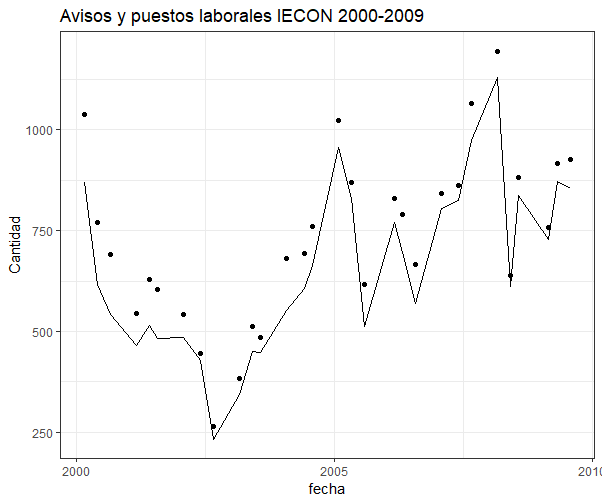
\includegraphics[width=\linewidth]{imagenes/chap4/iecon2000.png}
%		\caption{Avisos y Puestos IECON}
%	\end{subfigure}
%	\begin{subfigure}[b]{0.4\linewidth}
%		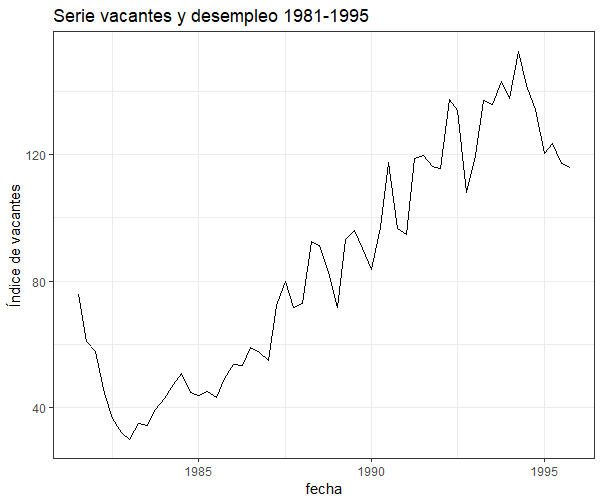
\includegraphics[width=\linewidth]{imagenes/chap4/VacantesUrrestarazu.png}
%		\caption{Vacantes Urrestarazu}
%	\end{subfigure}
%	\begin{subfigure}[b]{0.4\linewidth}
%		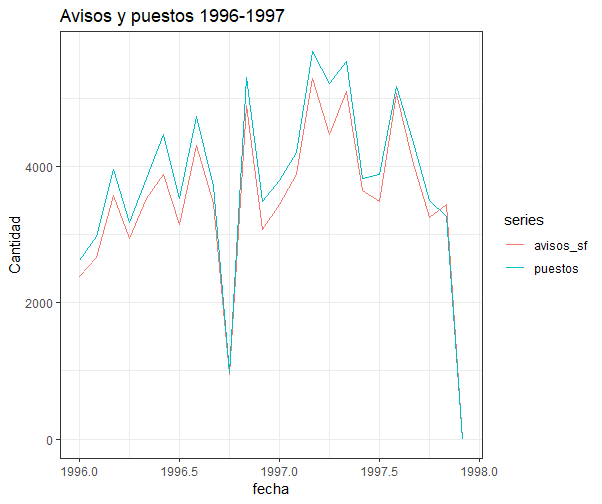
\includegraphics[width=\linewidth]{imagenes/chap4/MolinaAvisosyPuestos96.png}
%		\caption{Avisos recolectados 96-98}
%	\end{subfigure}
%	\begin{subfigure}[b]{0.4\linewidth}
%	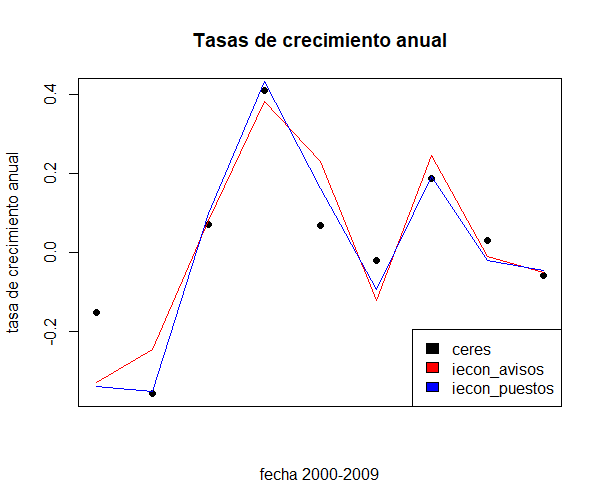
\includegraphics[width=\linewidth]{imagenes/chap4/CeresIECON2000.png}
%	\caption{Tasas crecimiento CERES-IECON}
%\end{subfigure}
%	\begin{subfigure}[b]{0.5\linewidth}
%		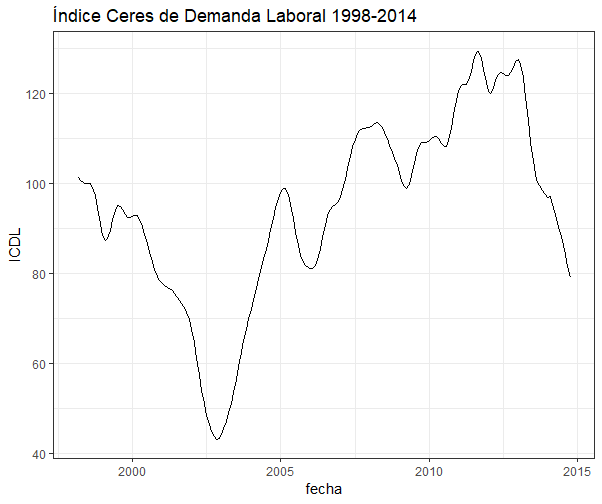
\includegraphics[width=\linewidth]{imagenes/chap4/ICDL98.png}
%		\caption{ICDL 1998-2014}
%	\end{subfigure}
%	\caption{Análisis de los datos obtenidos}
%	\label{fig:vacantes}
%\end{figure}

% PROBLEMÁTICAS

La serie de vacantes en proceso de construcción no esta exenta de críticas, las cuales vale destacar. La primera es que los datos solo permiten realizar un análisis para Montevideo, sin embargo, se encuentran sistemáticamente avisos laborales de otros departamentos del interior\footnote{Uruguay se compone de 19 grandes divisiones geográficas denominadas ``departamentos''. Por un lado esta Montevideo, y por el otro el resto de los 18 departamentos del país, lo que se denomina ``interior''.}, en especial de Maldonado y Canelones. Para el periodo recabado de 1995 a 1998 no se identifica cuantos avisos son y no son de Montevideo, sin embargo, si se logra obtener dicho número para el periodo de 2013-2018. En dicho caso los avisos publicados de otros departamentos oscilan en torno al 5\% del total publicaciones laborales. 

En segundo lugar, existe un claro sesgo hacia puestos laborales de baja calificación, lo cual se logra observar para el periodo 2013-2018 en base al análisis conjunto de la figura 2 y 3, donde se observa claramente que la mayor cantidad de avisos corresponden a puestos de auxiliar, técnico/especialista, ejecutivo comercial y peón. Esto va en linea con el resultado obtenido por \cite{Alma2011} para el periodo 2000-2010 utilizando la misma fuente de datos, quienes realizar un análisis pormenorizado de la información publicada en cada aviso laboral. Por lo cual, se supone que dicho sesgo también existe para el periodo 1980-1996.

%\begin{figure}[h]
%	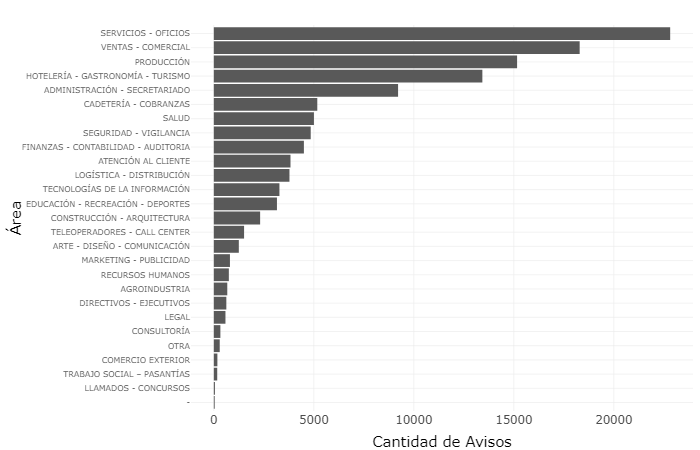
\includegraphics[width=\linewidth]{imagenes/chap4/newplot.png}
%	\caption{Cantidad de avisos laborales publicados en el diario El País, sección avisos laborales ``El Gallito'' entre 2013 y 2018. Los mismos son agrupados y ordenados de forma decreciente según el área en que se solicitan los avisos. El área, es una categoría propia del diario El País.}
%\end{figure}
%
%\begin{figure}[h]
%	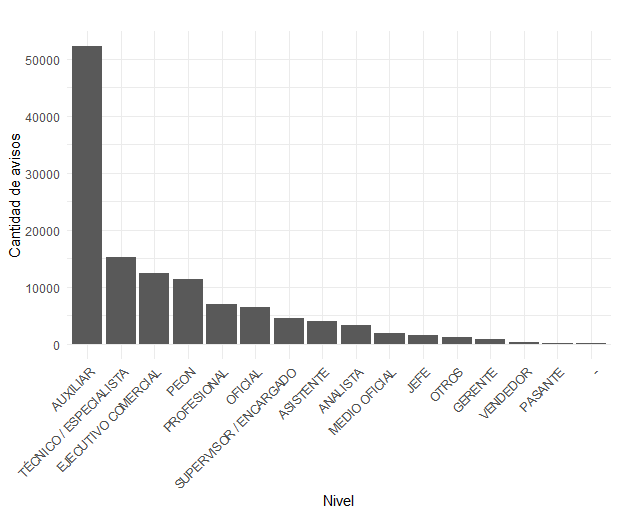
\includegraphics[width=\linewidth]{imagenes/chap4/gallito_nivel_2013_2018.png}
%	\caption{Cantidad de avisos laborales publicados en el diario El País, sección avisos laborales ``El Gallito'' entre 2013 y 2018. Los mismos son agrupados y ordenados de forma decreciente según el nivel jerárquico en que se solicitan los avisos. El nivel jerárquico, es una categoría propia del diario El País.}
%\end{figure}

En tercer lugar, la existencia de informalidad es una característica propia de los países subdesarrollados a la cual Uruguay y en específico Montevideo no escapa. Ello se agrava para los años entre 1980 y 2005, debido a las graves crisis económicas de 1982 y 2001-2002. Claramente las vacantes laborales publicadas en la prensa no captan los puestos generados en la informalidad.

Por último, ``El Gallito'' ha sido al menos hasta 2000-2010 el lugar predilecto por las empresas para publicar sus avisos laborales. Es un hecho incuestionable, por lo cual tomarlo como una muestra representativa de avisos laborales formales para el departamento de Montevideo es razonable. Sin embargo, con la penetración de Internet y la creación de portales de anuncios laborales como ``buscojobs'', ``computrabajo'', ``neuvo'' y ``linkedin'', entre otros, la competencia en el mercado de publicaciones ha aumentando considerablemente, no quedando claro en la actualidad cual es la página que reúne la mayor cantidad de avisos. Por esta razón, la representatividad del gallito ha disminuido y ello debe ser tenido en cuenta en el análisis, al menos desde 2009-2010 en adelante, dada la inserción de ``buscojobs'', ``computrabajo'' en torno a los años 2006-2007.

%\subsection{Estadísticas Descriptivas}

%[Presentar estadísticas descriptivas de los datos. Gráficos de las series, y al ser series temporales análisis estadísticas básicas de las series tales como test de R.U, de Raíz estacional, desestacionalización,]
